\documentclass[11pt]{article}
\usepackage[margin=1in]{geometry}
\usepackage{amsmath,amssymb}
\usepackage{graphicx}
\usepackage{booktabs}
\usepackage{xcolor}
\usepackage{hyperref}

\newcommand{\E}{\mathbb{E}}
\newcommand{\code}[1]{\texttt{#1}}

\title{The one-step-ahead predictive over time:\\ process variance, PIT and variance decomposition}
\author{Claude}
\date{October 9, 2026}

\emergencystretch=3em
\begin{document}
\maketitle

\section*{Summary}

This note follows the one-step-ahead predictive of the filter year by year, with and without
bias correction. It looks at three things: the learned process variance, the PIT, and a decomposition of the
predictive variance into process error and the other sources of variance. It asks whether
the PIT flattens as the filter learns a smaller process variance. It is a companion to
\code{claude-forecast-width-10.8.26}, which explains why the forecasts are too wide. It
reaches five conclusions.

\begin{enumerate}
  \item \textbf{With bias correction, the process variance falls steadily, by 20--50 times by 2017.} The median
  falls from 0.61 in 1991 to 0.01 (GEDI) and 0.03 (LandTrendr). Without correction it levels off at
  0.1--0.25 after about 1995.
  \item \textbf{The PIT flattens only a little, and only for GEDI.} For GEDI heteroskedastic
  $R$ the PIT interquartile range (IQR) widens from 0.22 in 1995 to 0.28 by 2000 and then stays at 0.29--0.30
  (calibrated: 0.5). For LandTrendr it does not widen at all (about 0.15--0.21), even though the
  process variance falls nine-fold over the same years.
  \item \textbf{The bias correction centres the PIT; it does not flatten it.} Corrected, the mean and median
  PIT sit at about 0.54 in every year. Uncorrected they sit at about 0.27--0.36.
  \item \textbf{The process variance stops mattering after the first few years.} The process share of the forecast variance
  is already small by the mid-1990s, so the remaining width comes from the
  observation error $R$, as shown in the forecast-width note.
  \item \textbf{Process error is 1--4\% of the predictive variance (median over sites) after 1995 with
  correction} (Section~\ref{sec:decomp}). The rest is the observation error $R$, the
  state uncertainty propagated from the previous analysis, and the disturbance part (the low tail
  from the disturbed mixture components). For LandTrendr, $R$ is 64--84\% of the
  variance. For GEDI heteroskedastic $R$, the disturbance part is the largest share (43--72\%).
  That tail inflates the variance but not the hump in the PIT.
\end{enumerate}

%================================================================================
\section{Runs and definitions}
\label{sec:defs}

\begin{itemize}
  \item \textbf{Runs.} The two full grids, without the disturbance product (so no year is
  flagged), at all 538 sites, for each of the four observation-error models:
  \begin{itemize}
    \item uncorrected: \code{experiments/fullRunNoBias};
    \item bias-corrected: \code{experiments/fullRunBias}, with
    \code{bias = list(rho = 0.9, denom = "N", skip = 1)}.
  \end{itemize}
  Year $t$ runs from 1991 to 2017. Year 1990 is excluded because its forecast starts
  from the population-wide prior on the initial state.
  \item \textbf{Process variance $v_{t-1}$.} The posterior mean of the process variance after assimilating
  $y_{t-1}$:
  \[
    v_{t-1} = \E[1/\tau \mid y_{1:t-1}] = \sum_g \pi_{t-1}(g)/\tau_g ,
  \]
  where $\pi_{t-1}(g)$ is the posterior weight of grid point $\tau_g$ (\code{hist\$procVar} at
  $t-1$). This is the process variance used by the forecast of $y_t$, so it is plotted at year
  $t$, aligned with that year's PIT. (\code{claude-forecast-width-10.8.26} plots $v_t$, the
  same series one year later.)
  \item \textbf{PIT $u_t$.} The probability integral transform of $y_t$ under its one-step-ahead
  predictive: the predictive probability of a value $\le y_t$ (\code{hist\$pit}). If
  the predictive is calibrated, $u_t$ is uniform on $[0,1]$: mean and median 0.5,
  quartiles 0.25 and 0.75, IQR 0.5. An IQR below 0.5 means the
  PIT is concentrated in the middle, i.e.\ the predictive is too wide. A median away from 0.5
  means it is biased (below 0.5: forecasts too high).
  \item \textbf{Across-site summaries.} For each year, the median, IQR (25th--75th
  percentile) and mean over the 538 sites, of $v_{t-1}$ and of $u_t$.
  \item \textbf{Coverage error of the central 50\% interval.} The fraction of sites with
  $|2u_t - 1| \le 0.5$ (the observation falls in the predictive's central 50\% interval),
  minus 0.5. Positive values mean the forecast is too wide; 0 means calibrated.
  \item \textbf{Periods.} 1991--95, 1996--2000, 2001--05, 2006--11 and 2012--17, for the PIT
  histograms in Figure~\ref{fig:periods}.
\end{itemize}

%================================================================================
\section{Process variance and PIT over time}
\label{sec:results}

\begin{figure}[p]
  \centering
  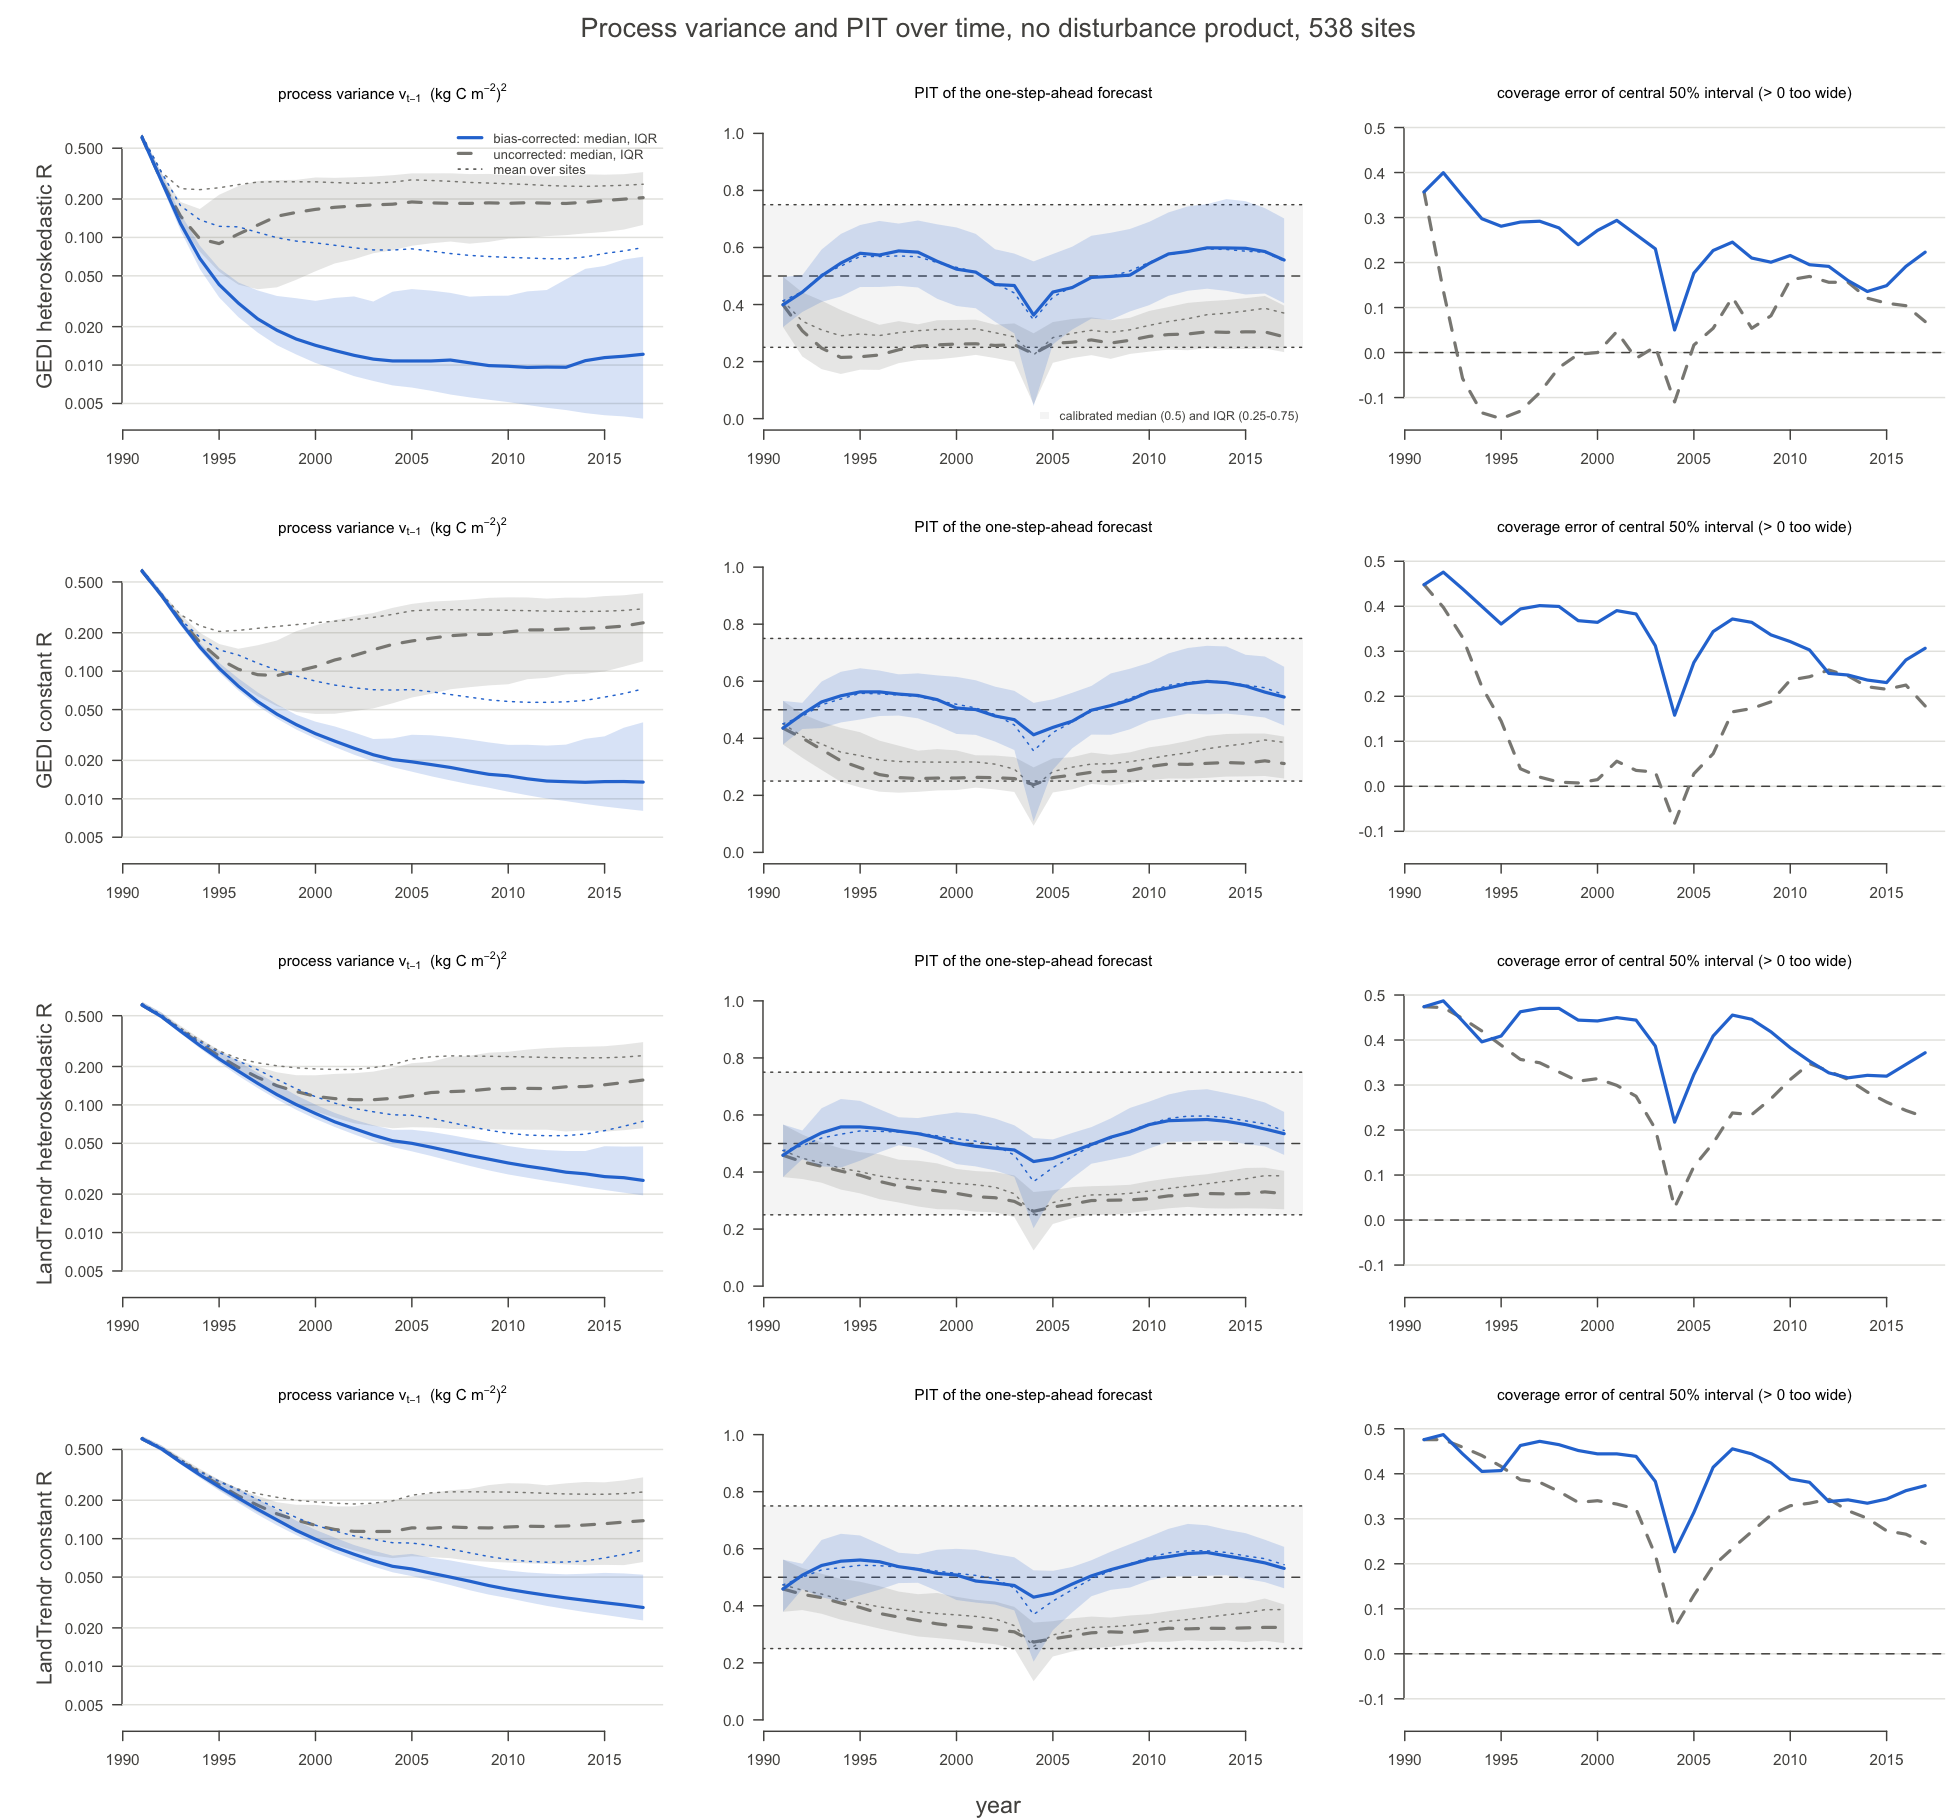
\includegraphics[width=\textwidth]{fw_pit_time.png}
  \caption{Per year, one row per observation-error model; blue = bias-corrected,
  gray dashed = uncorrected. \emph{Left:} process variance $v_{t-1}$ (log scale), median
  (thick line), IQR (band) and mean (dotted) over sites. \emph{Middle:} PIT $u_t$, median, IQR
  and mean over sites. The shaded strip and dotted lines at 0.25 and 0.75 are the calibrated
  quartiles. \emph{Right:} coverage error of the central 50\% interval.}
  \label{fig:time}
\end{figure}

\begin{figure}[p]
  \centering
  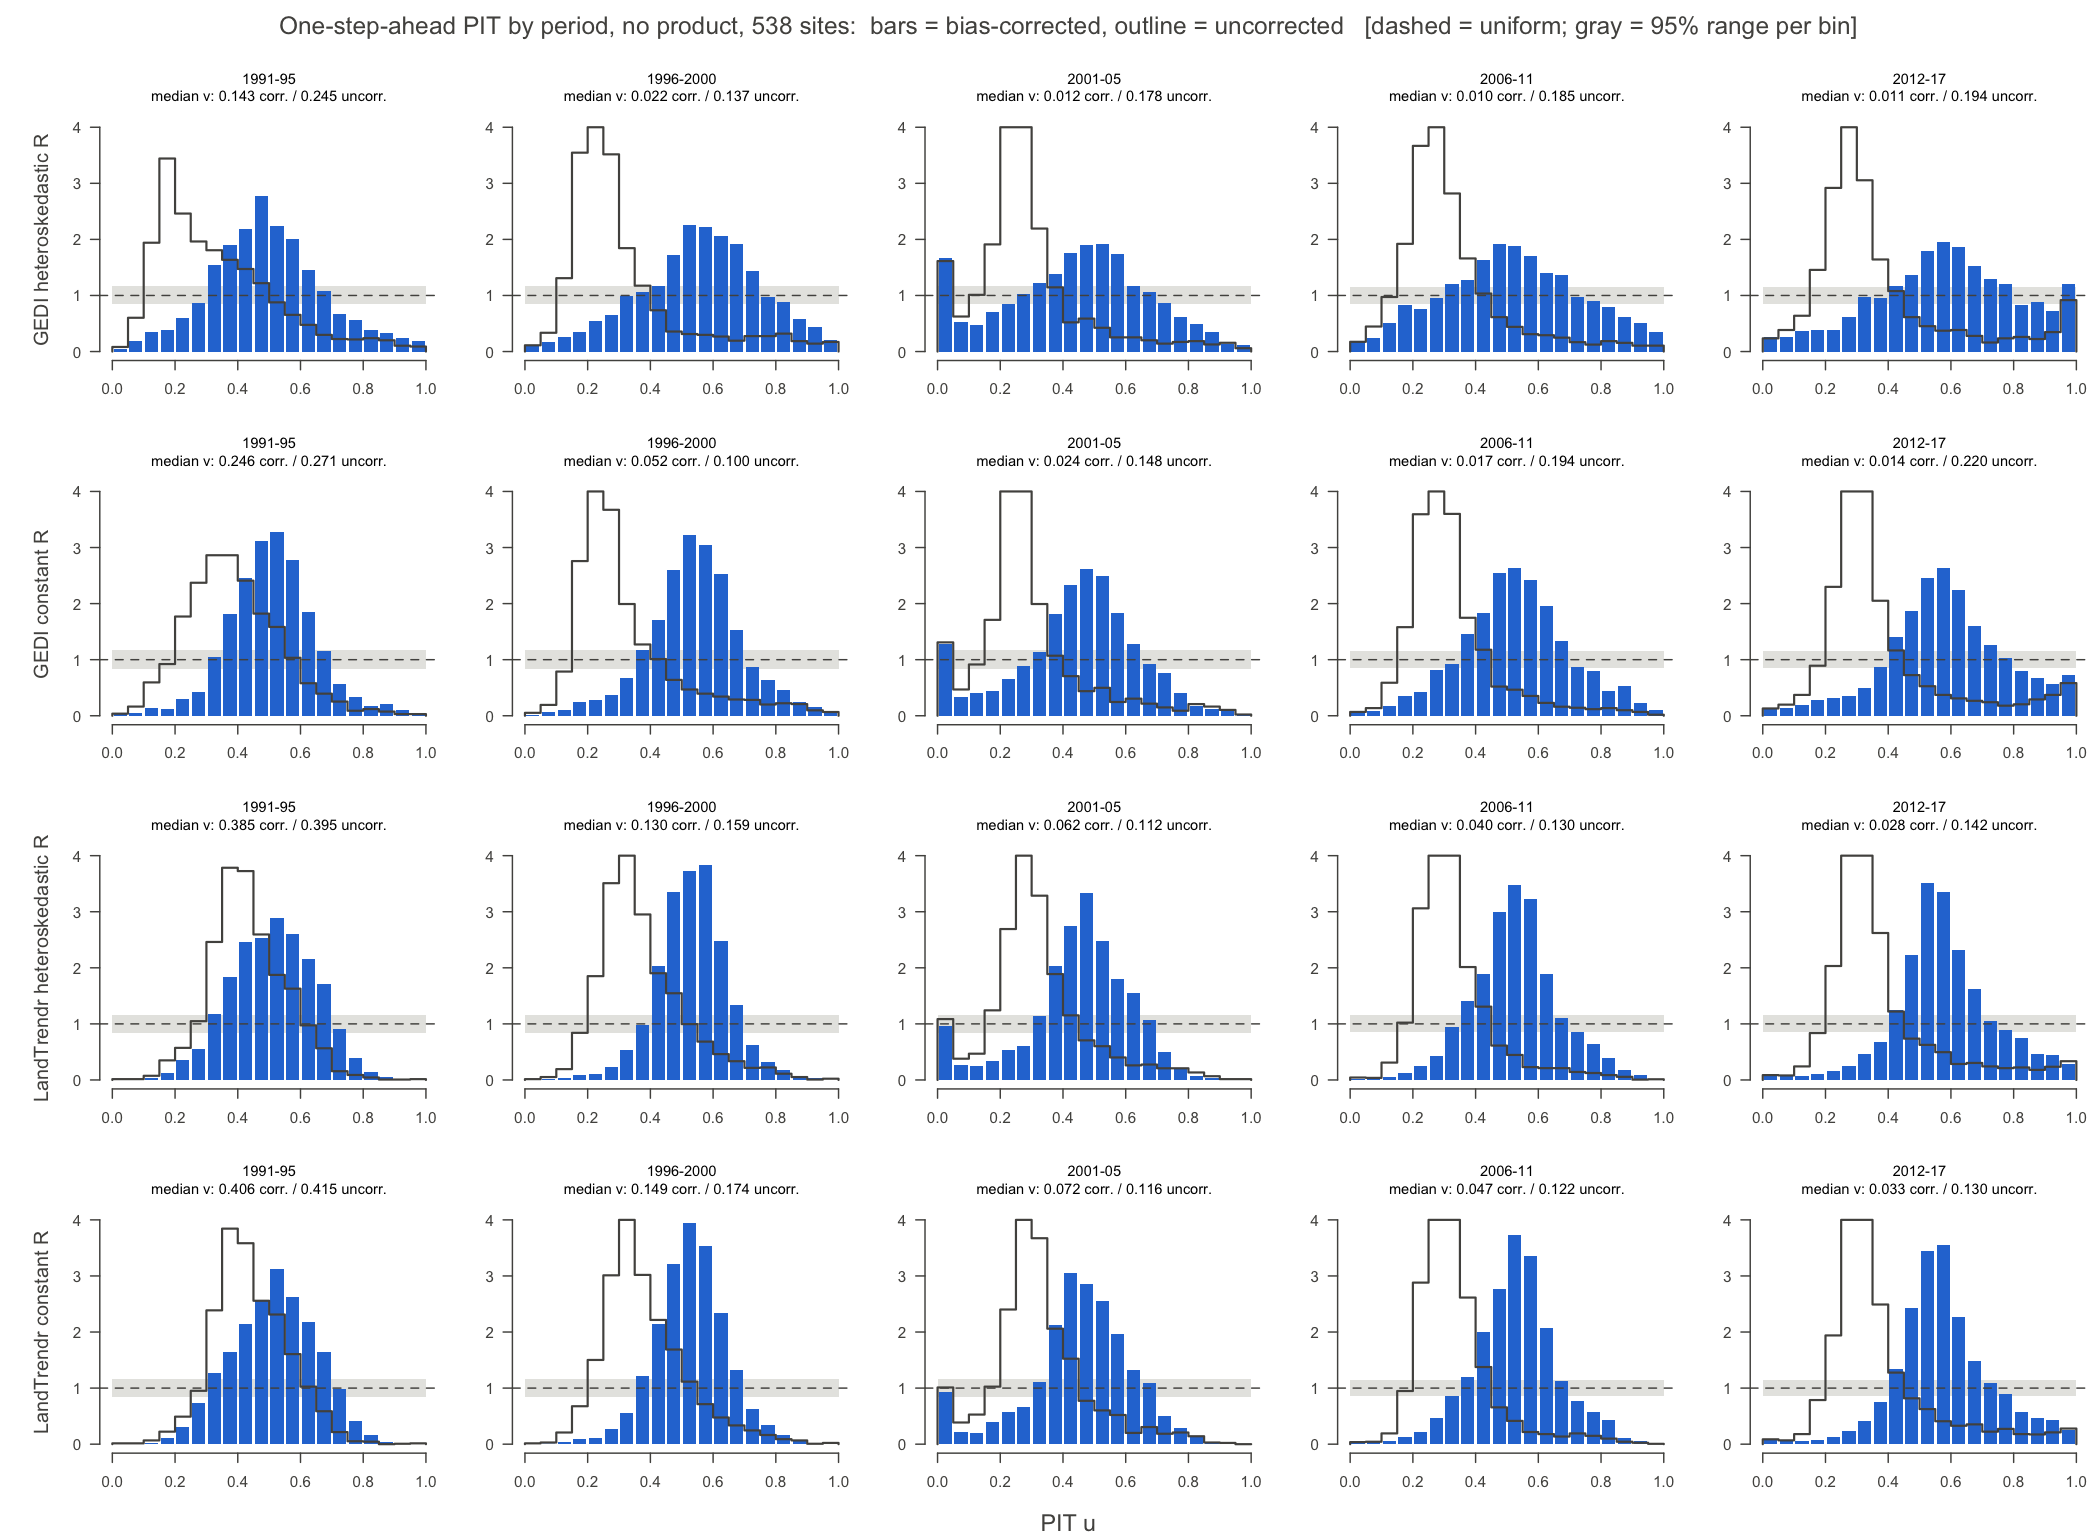
\includegraphics[width=\textwidth]{fw_pit_periods.png}
  \caption{PIT histograms by period (all sites and years in the period). Bars: bias-corrected;
  outline: uncorrected; dashed: uniform; gray: 95\% range of each bin under a uniform PIT.
  Panel titles give the median $v_{t-1}$ over the period.}
  \label{fig:periods}
\end{figure}

\begin{table}[ht]
  \centering\small
  \begin{tabular}{llrrrrrrr}
    \toprule
    & & \multicolumn{3}{c}{$v_{t-1}$} & \multicolumn{4}{c}{PIT $u_t$} \\
    \cmidrule(lr){3-5} \cmidrule(lr){6-9}
    model & year & median & IQR & mean & median & IQR & IQR width & cov.\ err.\ 50\% \\
    \midrule
    GEDI het.        & 1991 & 0.607 & 0.583--0.653 & 0.627 & 0.40 & 0.32--0.50 & 0.18 & 0.36 \\
                     & 1995 & 0.043 & 0.034--0.057 & 0.122 & 0.58 & 0.46--0.68 & 0.22 & 0.28 \\
                     & 2000 & 0.014 & 0.010--0.032 & 0.091 & 0.52 & 0.40--0.67 & 0.28 & 0.27 \\
                     & 2010 & 0.010 & 0.005--0.035 & 0.070 & 0.54 & 0.40--0.69 & 0.29 & 0.22 \\
                     & 2017 & 0.012 & 0.004--0.071 & 0.083 & 0.56 & 0.40--0.70 & 0.30 & 0.22 \\
    \addlinespace
    GEDI const.      & 1995 & 0.105 & 0.098--0.116 & 0.147 & 0.56 & 0.47--0.65 & 0.18 & 0.36 \\
                     & 2000 & 0.032 & 0.030--0.040 & 0.084 & 0.51 & 0.42--0.62 & 0.20 & 0.36 \\
                     & 2017 & 0.014 & 0.008--0.040 & 0.073 & 0.55 & 0.45--0.65 & 0.21 & 0.31 \\
    \addlinespace
    LandTrendr het.  & 1995 & 0.229 & 0.216--0.262 & 0.257 & 0.56 & 0.44--0.65 & 0.21 & 0.41 \\
                     & 2000 & 0.086 & 0.078--0.101 & 0.116 & 0.50 & 0.43--0.61 & 0.18 & 0.44 \\
                     & 2017 & 0.026 & 0.020--0.047 & 0.074 & 0.53 & 0.46--0.61 & 0.15 & 0.37 \\
    \addlinespace
    LandTrendr const.& 1995 & 0.255 & 0.238--0.288 & 0.280 & 0.56 & 0.44--0.65 & 0.21 & 0.41 \\
                     & 2000 & 0.099 & 0.090--0.117 & 0.128 & 0.51 & 0.42--0.60 & 0.18 & 0.44 \\
                     & 2017 & 0.029 & 0.023--0.052 & 0.082 & 0.53 & 0.46--0.61 & 0.15 & 0.37 \\
    \bottomrule
  \end{tabular}
  \caption{Bias-corrected runs, selected years: process variance $v_{t-1}$
  ((kg\,C\,m$^{-2}$)$^2$) and PIT over the 538 sites. Calibrated PIT: median 0.5, IQR
  0.25--0.75 (width 0.5), coverage error 0. Every year is in \code{fw\_pit\_time.csv}.}
  \label{tab:years}
\end{table}

\paragraph{Process variance (Figure~\ref{fig:time}, left).}
\begin{itemize}
  \item \textbf{With correction it keeps falling.} The median falls fastest in the first five
  years and keeps falling slowly after that. For GEDI it reaches about 0.01, for LandTrendr about 0.03 by 2017.
  \item \textbf{Without correction it levels off.} After about 1995 the uncorrected median stays at 0.1--0.25, and for GEDI it creeps up:
  the filter uses process variance to absorb the forecast bias (as in the forecast-width note).
  \item \textbf{The mean is much larger than the median and levels off at 0.06--0.13 after 2000.} The distribution
  over sites is right-skewed: most sites learn a small process variance, and a minority with
  large year-to-year jumps learn a much larger one. For GEDI heteroskedastic $R$ the upper
  quartile rises again after about 2013 (0.035 to 0.071), from sites whose biomass changes
  quickly late in the record.
\end{itemize}

\paragraph{PIT (Figure~\ref{fig:time}, middle and right; Figure~\ref{fig:periods}).}
\begin{itemize}
  \item \textbf{Centring: the correction works in every year.} Averaged over 1996--2017
  (excluding 2003--04, see below), the corrected mean PIT is 0.54 for every model.
  Uncorrected it is 0.33--0.36, with median 0.27--0.32: the uncorrected forecasts are too high
  throughout. The remaining 0.04 above 0.5 is the low disturbance tail of the predictive
  (forecast-width note, Section 3).
  \item \textbf{Concentration: the PIT flattens only a little, and only for GEDI.} For GEDI heteroskedastic $R$,
  the PIT IQR widens from 0.22 (1995) to 0.28 (2000) and then stays at 0.29--0.30, while
  the median $v_{t-1}$ falls only from 0.014 to 0.010. The central 50\% interval goes from 28 to 22
  points too wide. For GEDI constant $R$ the IQR stays at 0.18--0.21. For LandTrendr it
  \emph{narrows} slightly (0.21 to 0.15) even though $v_{t-1}$ falls nine-fold: the forecast
  errors shrink over time faster than the forecast variance, which stays dominated by $R$. In
  Figure~\ref{fig:periods} the corrected histograms stay humped in every period.
  \item \textbf{The uncorrected PIT can look better, by accident.} The uncorrected 50\% coverage error is near 0 or
  even negative for GEDI in 1995--2005. That is not calibration: the bias pushes the
  observations away from the centre of a predictive that is too wide, and the two errors partly cancel.
  The uncorrected PIT IQR is in fact narrower (0.13--0.15) than the corrected one.
  \item \textbf{2003--04 is a disturbance year.} Many sites lose biomass in 2003--04, which
  the undisturbed forecast does not expect. The PIT drops (median 0.36--0.44 corrected), its
  lower quartile falls to 0.04--0.20, and the coverage error dips. This is real disturbance,
  not better calibration, so it is excluded from the averages above.
  \item \textbf{A late tail toward high PIT.} From about 2010 the corrected GEDI histograms grow a tail toward
  $u_t = 1$, i.e.\ forecasts that are too low at some sites. This matches the regrowth
  over-correction seen at site 300: $b$ is learned in mature stands and is too negative for
  regrowing stands.
\end{itemize}

\paragraph{Interpretation.}
The process variance is the only part of the predictive variance that the filter learns,
and it does shrink. But after the first few years it is a small part of the predictive
variance (a median share of 1--4\% of the full predictive variance from 1996 on, against 17--83\% for $R$;
see \code{fw\_pit\_time.csv} and the forecast-width note). Once it is small, shrinking it further
cannot flatten the PIT. In the R-scaling experiment (\code{rs\_pit.png}), reducing $R$
flattens the PIT. That points to the observation-error model, not the process variance, as
the thing to change.

%================================================================================
\section{Decomposition of the predictive variance}
\label{sec:decomp}

\subsection{The one-step-ahead predictive}

At year $t$, before $y_t$ is assimilated, the filter's predictive for $y_t$ is a Gaussian
mixture over the $\tau$ grid points $g$, the two projected components $j \in \{1, 2\}$ and the
disturbance classes $k \in \{0, 1, \dots, D\}$ ($k = 0$: undisturbed):
\begin{equation}
  p(y_t \mid y_{1:t-1}) = \sum_{g,j,k} \omega_{gjk}\,
  \mathcal{N}\!\big(y_t;\ \mu_{gjk},\ s^2_{gjk}\big),
  \qquad
  s^2_{gjk} = \Sigma^F_{gjk,33} + R_t .
  \label{eq:pred}
\end{equation}
\begin{itemize}
  \item $\omega_{gjk} \propto \pi_{t-1}(g)\, w_{t-1}(g,j)\, \beta_{k,t}$, normalised to sum to 1.
  Here $\pi_{t-1}(g)$ is the $\tau$ posterior after $y_{t-1}$, $w_{t-1}(g,j)$ is the weight of
  projected component $j$ at grid point $g$, and $\beta_{k,t}$ is the prior probability of class
  $k$ in year $t$. Components whose importance weights are degenerate get $\omega = 0$.
  \item $\mu_{gjk}$ is the forecast mean of the wood pool: VSEM run from the previous analysis,
  then the disturbance draw for $k \ge 1$. With bias correction, $\mu_{gj0}$ includes the
  shift $b_t$.
  \item $\Sigma^F_{gjk,33}$ is the forecast variance of the wood pool. For $k = 0$ it is
  $\sigma^2_{gj0} + 1/\tau_g$, where $\sigma^2_{gj0}$ is the importance-weighted ensemble
  variance of the VSEM forecast and $1/\tau_g$ the process variance. For $k \ge 1$ it is the ensemble
  variance after the disturbance draw, with no process variance added.
  \item $R_t$ is the observation-error variance.
\end{itemize}
The PIT of Section~\ref{sec:defs} is $u_t = \sum_{g,j,k} \omega_{gjk}\,\Phi\big((y_t - \mu_{gjk})/s_{gjk}\big)$,
where $\Phi$ is the standard normal CDF. The predictive mean and variance are
\begin{equation}
  m_t = \sum_{g,j,k} \omega_{gjk}\,\mu_{gjk}, \qquad
  V_t = \sum_{g,j,k} \omega_{gjk}\big(s^2_{gjk} + \mu^2_{gjk}\big) - m_t^2
  \qquad (\code{predVar}).
  \label{eq:V}
\end{equation}

\subsection{Splitting by disturbance class}

Group the components by $k$. Class $k$ has total weight $\beta^k = \sum_{g,j}\omega_{gjk}$
(equal to $\beta_{k,t}$ when no component is dropped), within-class weights
$\omega^k_{gj} = \omega_{gjk}/\beta^k$, and within-class mean and variance
\[
  m^k = \sum_{g,j}\omega^k_{gj}\,\mu_{gjk}, \qquad
  V^k = \sum_{g,j}\omega^k_{gj}\big(s^2_{gjk} + \mu^2_{gjk}\big) - (m^k)^2 .
\]
The law of total variance gives
\begin{equation}
  V_t = \underbrace{\beta^0 V^0}_{\text{undisturbed}}
      + \sum_{k \ge 1}\beta^k V^k
      + \sum_{k \ge 0}\beta^k\,(m^k - m_t)^2 .
  \label{eq:ltv}
\end{equation}
The undisturbed class is the no-disturbance predictive of the forecast-width note:
$m^0$ = \code{predMean0}, $V^0$ = \code{predVar0}. Its variance splits into
\begin{equation}
  V^0 = R_t + Q^0_t + P^0_t, \qquad
  Q^0_t = \sum_{g,j}\omega^0_{gj}/\tau_g \ (\code{predProcVar0}), \qquad
  P^0_t = \sum_{g,j}\omega^0_{gj}\,\sigma^2_{gj0} + \sum_{g,j}\omega^0_{gj}\,(\mu_{gj0} - m^0)^2 .
  \label{eq:V0}
\end{equation}
$Q^0_t$ is the process variance, averaged over the $\tau$ posterior. $P^0_t$ is the
\emph{propagated state variance}: the analysis uncertainty carried through VSEM, plus the
spread of the component means. In the code $P^0_t = V^0 - R_t - Q^0_t$.

\subsection{The decomposition}

Every component contains $R_t$, so $\sum_k \beta^k R_t = R_t$. Pulling $R_t$ out of
\eqref{eq:ltv} and splitting $\beta^0 V^0$ with \eqref{eq:V0} gives an exact four-way
decomposition:
\begin{equation}
  \boxed{\;V_t = \underbrace{R_t}_{\text{observation error}}
  + \underbrace{\beta^0 Q^0_t}_{\text{process error}}
  + \underbrace{\beta^0 P^0_t}_{\text{propagated state}}
  + \underbrace{D_t}_{\text{disturbance}}\;}
  \label{eq:decomp}
\end{equation}
\begin{equation}
  D_t = \sum_{k \ge 1}\beta^k\,(V^k - R_t) + \sum_{k \ge 0}\beta^k\,(m^k - m_t)^2
      = V_t - R_t - \beta^0\,(V^0 - R_t) .
  \label{eq:D}
\end{equation}
\begin{itemize}
  \item \textbf{Disturbance part $D_t$.} The variance from allowing a disturbance: the forecast spread of the disturbed
  classes, plus the spread between the class means. The undisturbed and disturbed means can be
  several kg\,C\,m$^{-2}$ apart.
  \item \textbf{Process error $\beta^0 Q^0_t$.} This is \code{predProcVar}. It is the only term that contains $1/\tau$, so it is
  the only part of the predictive variance the $\tau$ posterior controls directly. ($P^0_t$
  depends on $\tau$ indirectly, through earlier analyses.)
  \item \textbf{How it is computed.} From stored outputs: $\beta^0 = \code{predProcVar}/\code{predProcVar0}$, $R_t$ =
  \code{predR}, and $D_t$ from \eqref{eq:D}. The script checks that the four parts sum to
  $V_t$ (to $10^{-8}$).
  \item \textbf{Summaries.} Figure~\ref{fig:decomp} shows the mean of each term over sites. Means add up, so
  the stack equals the mean $V_t$. Figure~\ref{fig:share} shows the median over sites of each term's
  share of $V_t$. Medians do not add up, but they are not dominated by the few sites with
  very large $Q^0_t$.
  \item \textbf{Data.} $\code{predVar0}$ and $\code{predProcVar0}$ are only stored by the 100-site subset reruns
  (\code{experiments/forecastWidth}), so this section uses those 100 sites, both runs, no
  product. Without the product, $\beta^0 = 0.954$, the background probability of no disturbance.
\end{itemize}

\subsection{Results}

\begin{figure}[p]
  \centering
  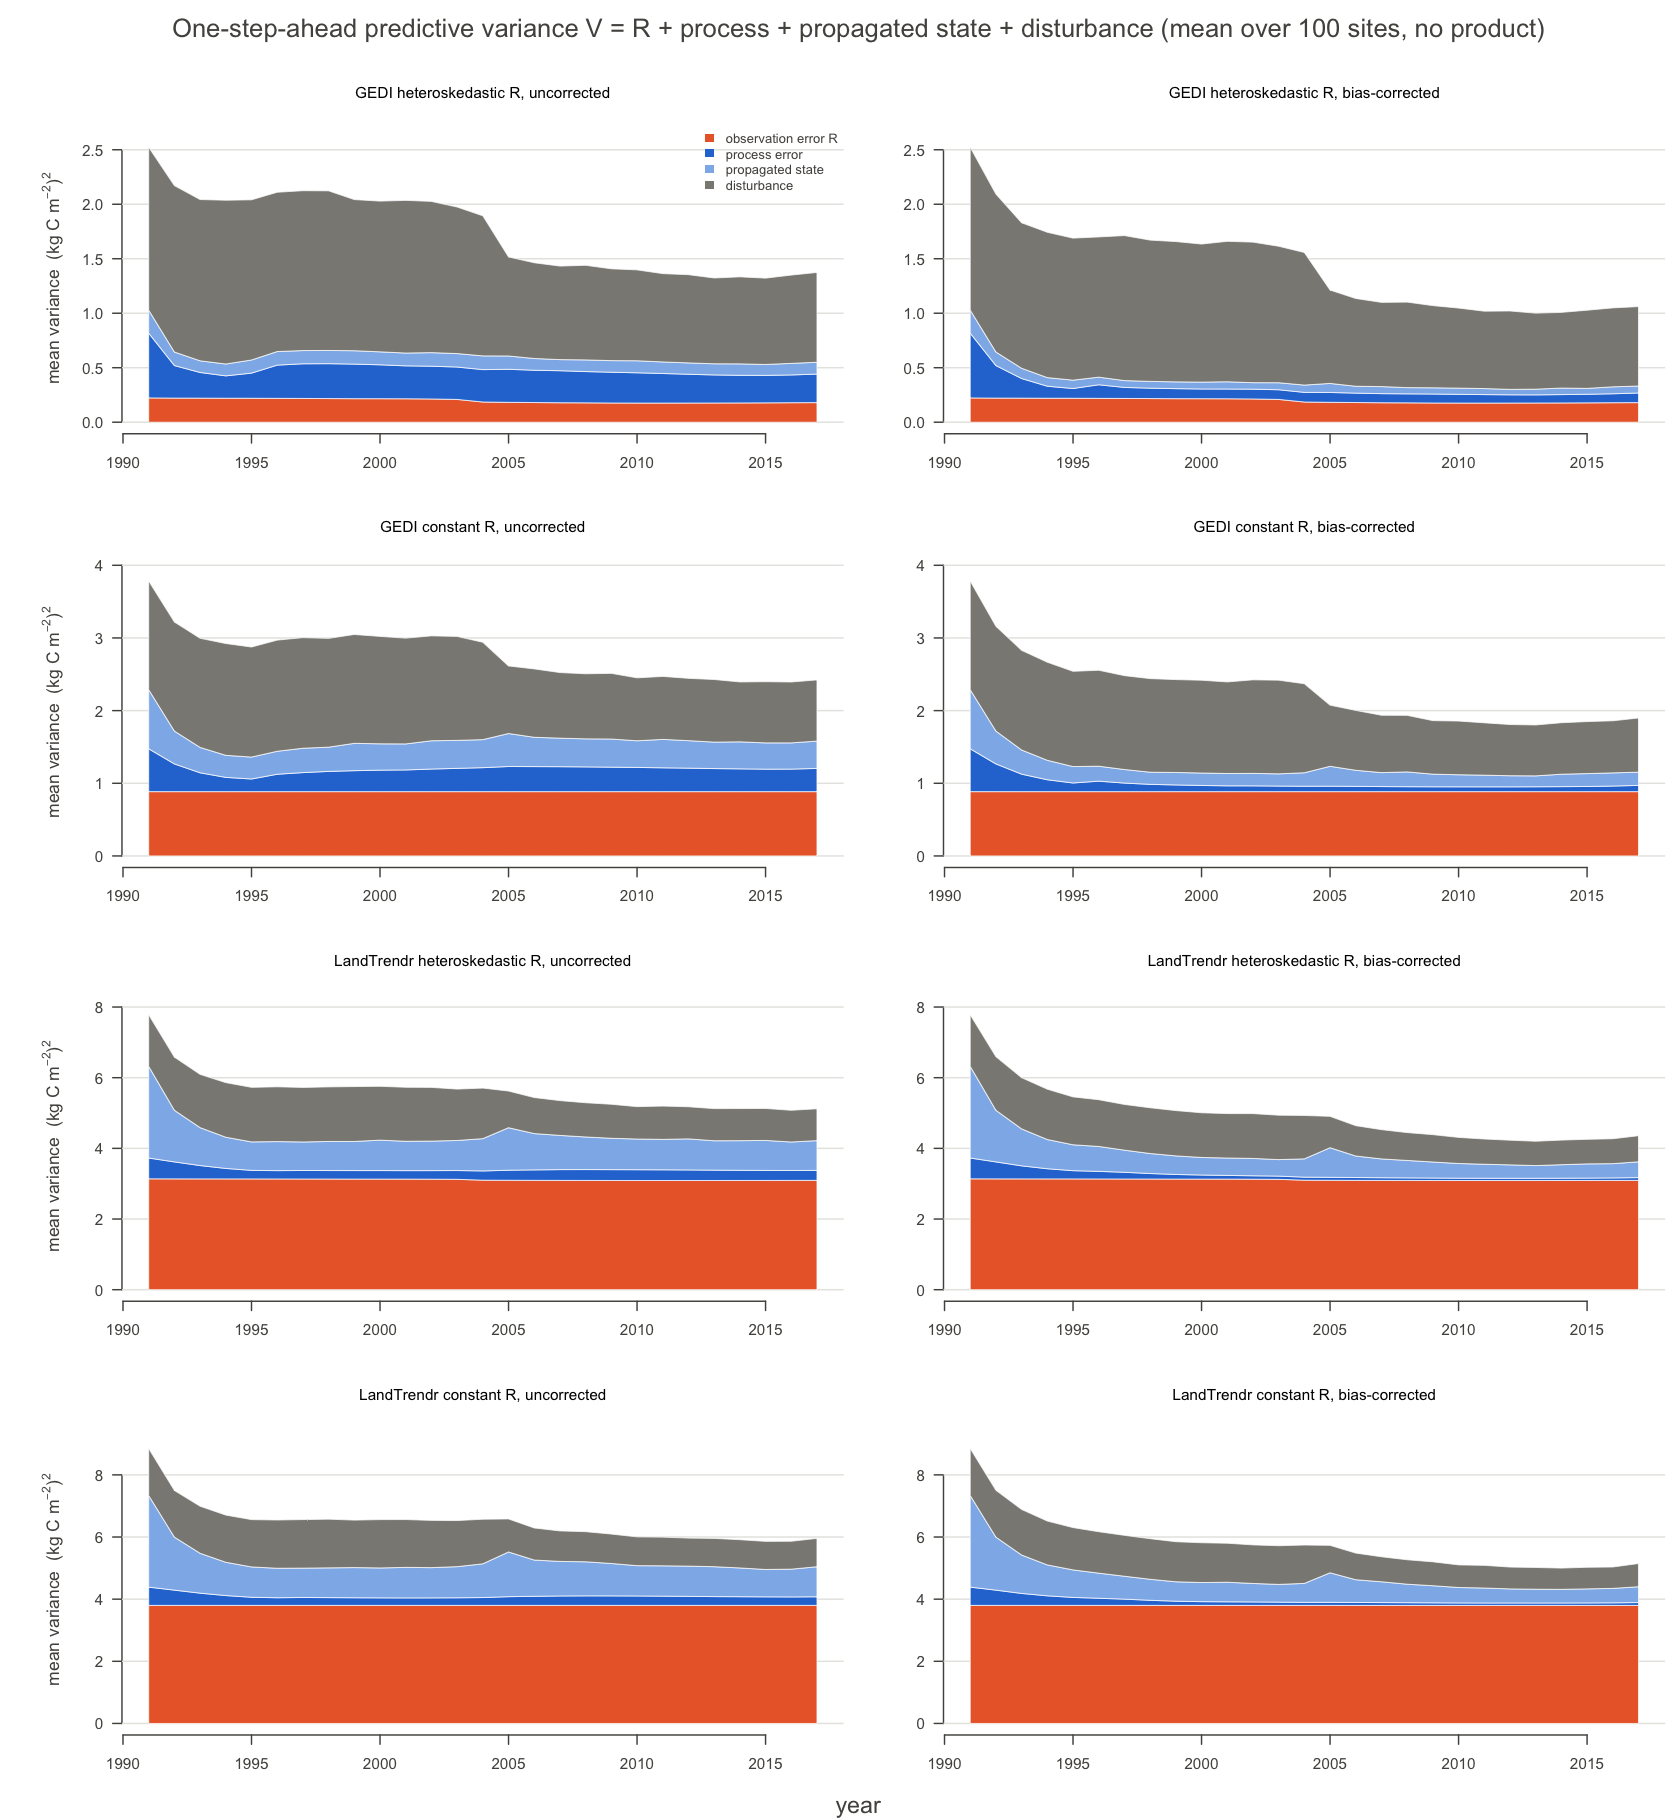
\includegraphics[width=0.92\textwidth]{fw_var_decomp.png}
  \caption{Decomposition \eqref{eq:decomp} of the one-step-ahead predictive variance $V_t$,
  mean over the 100 sites in each year, stacked. Rows: observation-error model; columns:
  uncorrected, bias-corrected. Note the different $y$-axis ranges per row.}
  \label{fig:decomp}
\end{figure}

\begin{figure}[ht]
  \centering
  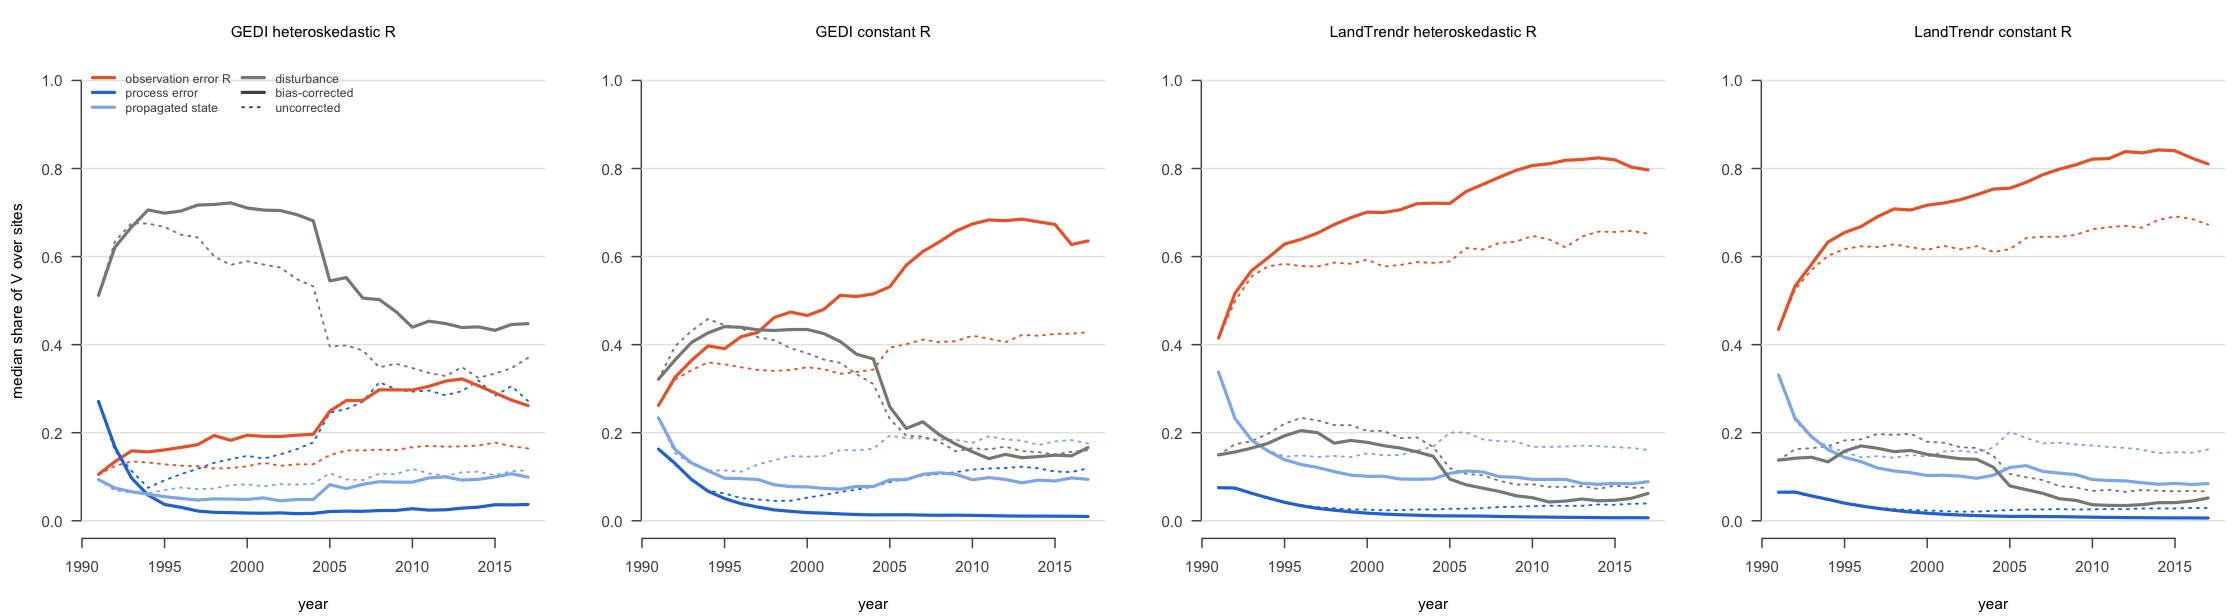
\includegraphics[width=\textwidth]{fw_var_share.png}
  \caption{Median over the 100 sites of each term's share of $V_t$. Solid: bias-corrected;
  dotted: uncorrected.}
  \label{fig:share}
\end{figure}

\begin{table}[ht]
  \centering\small
  \begin{tabular}{llrrrrr}
    \toprule
    model & run & $V_t$ & $R_t$ & $\beta^0 Q^0_t$ & $\beta^0 P^0_t$ & $D_t$ \\
    \midrule
    GEDI het.         & uncorr. & 1.32--2.12 & 0.18--0.22 & 0.25--0.32 & 0.10--0.13 & 0.79--1.47 \\
                      & corr.   & 1.00--1.71 & 0.18--0.22 & 0.07--0.12 & 0.05--0.08 & 0.69--1.33 \\
    GEDI const.       & uncorr. & 2.39--3.05 & 0.88       & 0.24--0.35 & 0.32--0.45 & 0.82--1.53 \\
                      & corr.   & 1.80--2.56 & 0.88       & 0.07--0.14 & 0.15--0.27 & 0.70--1.32 \\
    LandTrendr het.   & uncorr. & 5.08--5.76 & 3.09--3.13 & 0.24--0.31 & 0.81--1.20 & 0.90--1.55 \\
                      & corr.   & 4.20--5.38 & 3.09--3.13 & 0.06--0.22 & 0.36--0.84 & 0.69--1.32 \\
    LandTrendr const. & uncorr. & 5.86--6.58 & 3.80       & 0.24--0.31 & 0.88--1.44 & 0.90--1.57 \\
                      & corr.   & 5.00--6.17 & 3.80       & 0.08--0.23 & 0.44--0.95 & 0.68--1.33 \\
    \midrule
    \multicolumn{2}{l}{median share, corrected} & & & & & \\
    GEDI het.         & & & 17--32\% & 2--4\% & 5--11\% & 43--72\% \\
    GEDI const.       & & & 42--69\% & 1--4\% & 7--11\% & 14--44\% \\
    LandTrendr het.   & & & 64--82\% & 1--3\% & 8--13\% & 4--20\% \\
    LandTrendr const. & & & 67--84\% & 1--3\% & 8--13\% & 3--17\% \\
    \bottomrule
  \end{tabular}
  \caption{Range over 1996--2017 of the mean (over sites) of each term ((kg\,C\,m$^{-2}$)$^2$),
  and of the median share of $V_t$ for the corrected runs. Every year is in
  \code{fw\_var\_decomp.csv}.}
  \label{tab:decomp}
\end{table}

\begin{itemize}
  \item \textbf{Process error is small, and the correction makes it smaller.} With correction the mean process term falls
  from about 0.59 in 1991 to 0.06--0.14 from 1996 on, against 0.24--0.35 uncorrected. Its median
  share of $V_t$ is 1--4\%. This is the term the PIT-over-time results (Section~\ref{sec:results}) follow, and it is too
  small to matter by the late 1990s.
  \item \textbf{$R_t$ is fixed, so its share grows as the other terms shrink.} It does not change with
  correction (apart from the small $y_t$ dependence of the heteroskedastic models). As the
  process and propagated-state terms shrink, its share rises: for LandTrendr from 41\% (1991) to
  80--84\% (2010s), for GEDI constant $R$ to 64--69\%.
  \item \textbf{The propagated state term is large for LandTrendr.} It is 0.36--0.95 corrected, against 0.05--0.08 for
  GEDI heteroskedastic. With a large $R$ the analysis barely shrinks the state uncertainty, so it is carried
  forward (forecast-width note, Section~3). The correction roughly halves it.
  \item \textbf{The disturbance part is the same for every observation-error model.} Its mean is about 1.28 before
  2005 and 0.75 after, for all four. It does not depend on $R$: it is set by the background disturbance
  probability $1 - \beta^0 = 0.046$ and by how far the disturbed means sit below the undisturbed
  one, which scales with the biomass present. The drop after 2004 follows the 2003--04 disturbances,
  which left many sites with less biomass to lose. For GEDI heteroskedastic $R$, where every
  other term is small, it is the largest share of $V_t$ (43--72\%).
  \item \textbf{Why the disturbance part does not cause the hump.} $D_t$ is variance held by a
  tail with only 4.6\% of the probability, several kg\,C\,m$^{-2}$ below the undisturbed
  forecast. For an undisturbed year, $u_t \approx (1 - \beta^0) + \beta^0\,
  \Phi\big((y_t - m^0)/\sqrt{V^0}\big)$, so the tail only shifts the PIT up by at most 0.046 (the
  which accounts for most of the gap between 0.5 and the 0.54 mean PIT of Section~\ref{sec:results}). How concentrated the PIT is depends on $V^0 = R_t + Q^0_t + P^0_t$
  relative to the actual errors. In that part, $R_t$ dominates once $Q^0_t$ is small.
\end{itemize}

%================================================================================
\section*{Reproducing}

\code{Rscript claude-working-docs/forecast\_width\_analysis.R}, from the repository root,
with \code{EXP\_DIR} set if the experiment folders are elsewhere. Section 6 of the script
writes \code{fw\_pit\_time.png}, \code{fw\_pit\_periods.png} and \code{fw\_pit\_time.csv}.
Section 7 writes \code{fw\_var\_decomp.png}, \code{fw\_var\_share.png} and
\code{fw\_var\_decomp.csv}; it uses the 100-site subset reruns in
\code{experiments/forecastWidth}, which section 2 creates if they are missing.

\end{document}
